%%%%%%%%%%%%%%%%%%%%%%%%%%%%%%%%%%%%%%%%%
% University Assignment Title Page 
% LaTeX Template
% Version 1.0 (27/12/12)
%
% This template has been downloaded from:
% http://www.LaTeXTemplates.com
%
% Original author:
% WikiBooks (http://en.wikibooks.org/wiki/LaTeX/Title_Creation)
%
% License:
% CC BY-NC-SA 3.0 (http://creativecommons.org/licenses/by-nc-sa/3.0/)
% 
% Instructions for using this template:
% This title page is capable of being compiled as is. This is not useful for 
% including it in another document. To do this, you have two options: 
%
% 1) Copy/paste everything between \begin{document} and \end{document} 
% starting at \begin{titlepage} and paste this into another LaTeX file where you 
% want your title page.
% OR
% 2) Remove everything outside the \begin{titlepage} and \end{titlepage} and 
% move this file to the same directory as the LaTeX file you wish to add it to. 
% Then add \input{./title_page_1.tex} to your LaTeX file where you want your
% title page.
%
%%%%%%%%%%%%%%%%%%%%%%%%%%%%%%%%%%%%%%%%%
%\title{Title page with logo}
%----------------------------------------------------------------------------------------
%	PACKAGES AND OTHER DOCUMENT CONFIGURATIONS
%----------------------------------------------------------------------------------------

\documentclass[12pt]{article}
\usepackage[english]{babel}
\usepackage[utf8x]{inputenc}
\usepackage{amsmath}
\usepackage{graphicx}
\usepackage[colorinlistoftodos]{todonotes}

\begin{document}

\begin{titlepage}

\newcommand{\HRule}{\rule{\linewidth}{0.5mm}} % Defines a new command for the horizontal lines, change thickness here

\center % Center everything on the page
 
%----------------------------------------------------------------------------------------
%	HEADING SECTIONS
%----------------------------------------------------------------------------------------

\textsc{\LARGE Politecnico di Milano}\\[1.5cm] % Name of your university/college
\textsc{\Large Dipartimento Elettronica, Informazione e Bioingegneria}\\[0.5cm] % Major heading such as course name
\textsc{\large HEAPLab Project Report}\\[0.5cm] % Minor heading such as course title

%----------------------------------------------------------------------------------------
%	TITLE SECTION
%----------------------------------------------------------------------------------------

\HRule \\[0.4cm]
{ \huge \bfseries SchedSim}\\[0.4cm] % Title of your document
\HRule \\[1.5cm]
 
%----------------------------------------------------------------------------------------
%	AUTHOR SECTION
%----------------------------------------------------------------------------------------

\begin{minipage}{0.4\textwidth}
\begin{flushleft} \large
\emph{Author:}\\
\textsc{Francesco Ratti} % Your name
\end{flushleft}
\end{minipage}
~
\begin{minipage}{0.4\textwidth}
\begin{flushright} \large
\emph{Supervisor:} \\
\textsc{Dr. Giusppe Massari} % Supervisor's Name
\end{flushright}
\end{minipage}\\[2cm]

% If you don't want a supervisor, uncomment the two lines below and remove the section above
%\Large \emph{Author:}\\
%John \textsc{Smith}\\[3cm] % Your name

%----------------------------------------------------------------------------------------
%	DATE SECTION
%----------------------------------------------------------------------------------------

{\large 21/03/2021}\\[2cm] % Date, change the \today to a set date if you want to be precise

%----------------------------------------------------------------------------------------
%	LOGO SECTION
%----------------------------------------------------------------------------------------


\includegraphics[width=100pt]{heaplogo.pdf}\\[1cm] % Include a department/university logo - this will require the graphicx package
 
%----------------------------------------------------------------------------------------

\vfill % Fill the rest of the page with whitespace

\end{titlepage}

\section{Introduction}

This application is a real time schedulers simulator developed using Python and PyQt for the GUI.

Given a set of tasks, which can be defined in the program and can be imported/exported as XML, SchedSim provides as output a list of temporally ordered events, in CSV format, ready to be displayed in a temporal chart. This tool can be useful for simulating new types of schedulers (for research purposes for example) and, subsequently, visualize the results starting from the "event list" output file by means of an external application.
\newline
Output event code is described in the dedicated section. 
\par SchedSim provides a simple interface (abstract class) which can be implemented to allow user to include his/her own scheduling algorythm. Deadline Monotonic algorythm is built-in and provided as a working example. 

\section{Design and Implementation}

All the GUI classes and method are in the main.py file. Other functions are splitted in the corresponding files, as later described.
\par SchedIo.py contains all inputs and outputs functions needed to import and export to XML file the tasks set and SchedEventWriter, which is used to write the output file. More details later.

\begin{center}
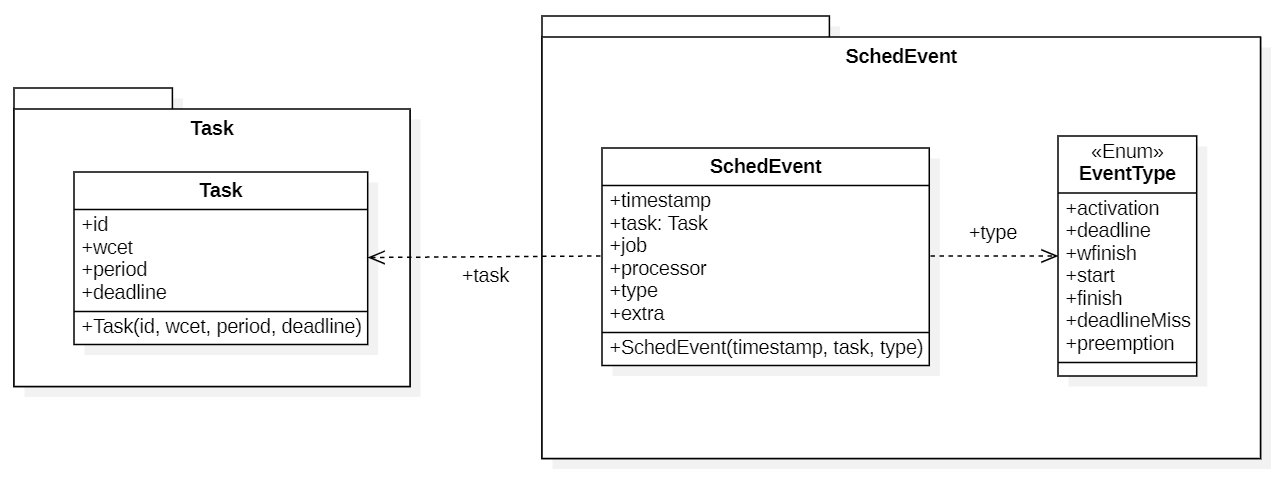
\includegraphics[width=1\textwidth]{SchedEventClass.png}
\end{center}
SchedEvent.py contains SchedEvent class, the one dedicated to time events, which will be exported in the output file, and an enum to set the code which corresponds to the given event. SchedEvent represent an event, associated to a timestamp, which will be part of the output list of temporally ordered events. In the current version, job, processor and extra are set to 0 but they can be easily implemented in future versions by adding these parameters in the SchedEvent class constructor.
\par Tasks.py contains Task class, which represent a single task with its attributes.

\begin{center}
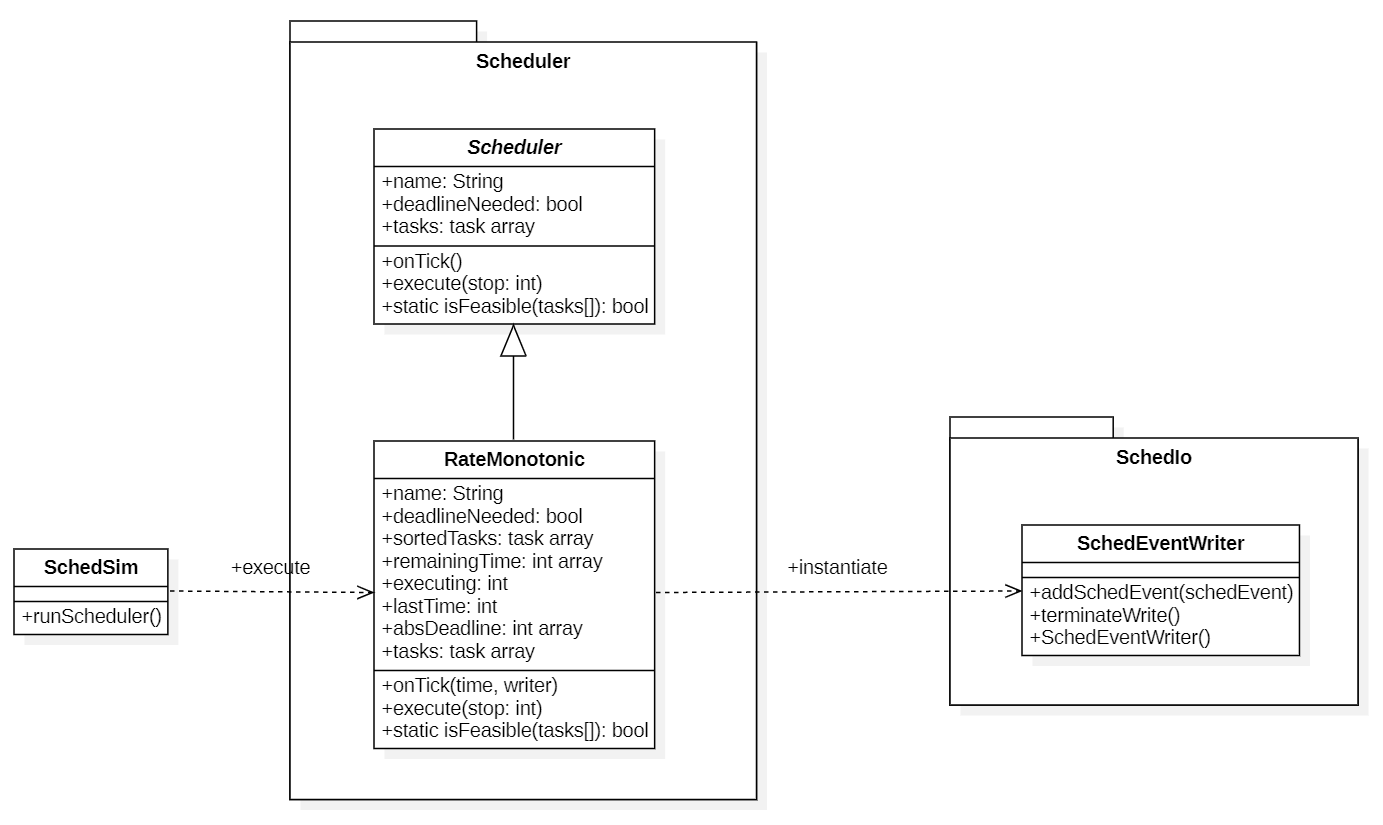
\includegraphics[width=1\textwidth]{SchedulerClass.png}
\end{center}
Scheduler.py contains the core of the system: all the scheduling algorythms are located there. In particular, one can add his/her own schedulers by extending Scheduler class, overriding execute and onTick methods and adding the corresponding scheduler class name in the "schedulers" variable (an array) in the file. Moreover, when extending Scheduler class one must override "name" and "deadlineNeeded", which must be set to true when it is mandatory that the user specifies a deadline for every task when using the given scheduler. For instance, it is set to false for RateMonotonic scheduler. It is needed to override "isFeasible" method too, which should return a boolean value. This method will be called by SchedSim to check whether the scheduling is feasible before actually executing it by means of calling "execute"; if it is not, an error message is shown.

\begin{center}
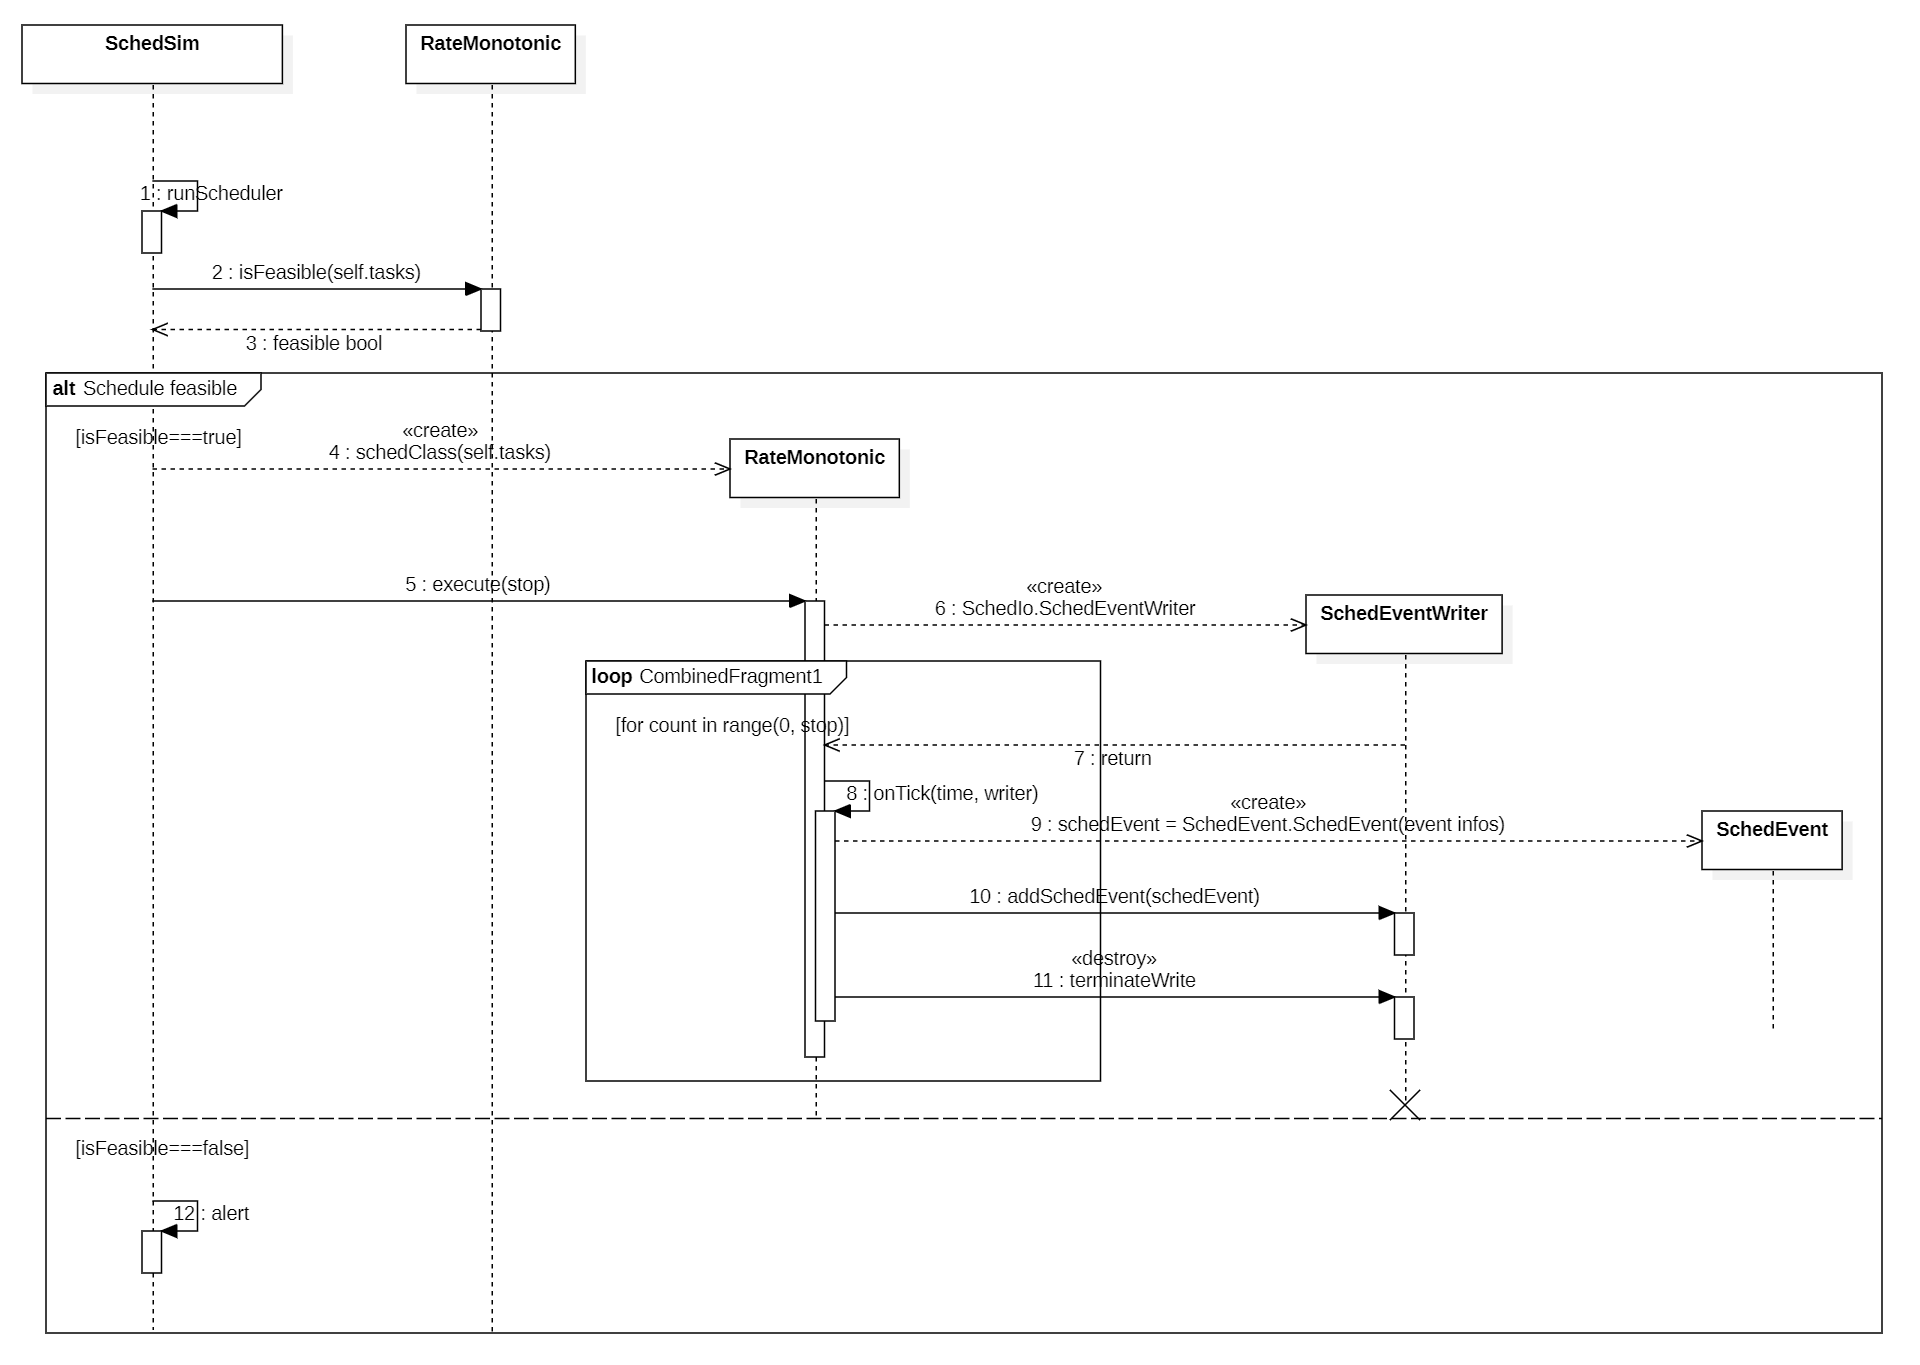
\includegraphics[width=1\textwidth]{SchedulerSequence.png}
\end{center}
runScheduler method, which is part of SchedSim class (main GUI class), is run when user clicks "Run" button. "isFeasible" inside the selected scheduler class is the called to check schedule feasibility and iff schedule is feasible, scheduler is istantated and execute is called. SchedEventWriter class is instantiated inside "execute" and "onTick" method, it will produce the scheduled events output file. When an event occours a SchedEvent is instantiated and SchedEventWriterinstance.addSchedEvent(schedEvent) is called. At the end, SchedEventWriterinstance.terminateWrite() is called to write the file.

\section{Input and output}
\subsection{Exported task set file structure}
Example of exported task set as XML by means of "Export" function:
\begin{verbatim}
<simulation>
<software>
<tasks>
<periodictask id="1" period="10" deadline="-1" wcet="2" />
<periodictask id="2" period="60" deadline="-1" wcet="10" />
<periodictask id="3" period="30" deadline="-1" wcet="5" />
</tasks>
</software>
</simulation>
\end{verbatim}
\subsection{Output file format}
Each line of the CSV file represents an event and it is composed of 6 fields:
\begin{verbatim}
timestamp,task,job,processor,type_of_event,extra_data
\end{verbatim}
where:


\begin{itemize}
    \item timestamp: the elapsed time since the epoch of measurements (usually 0). 
This can be measured in different time units (e.g. seconds,
milliseconds, clock cycles, etc.). This may not be unique in
the file, multiple events may happen at the same time.
    \item  task: the task id. If the event refers to a processor-only event, this value is 0.
    \item job: the job id. If the event refers to a processor-only event, this value is 0.
    \item processor: the processor id where the event happened. If the event is not processor-related, this value is 0.
    \item type\_of\_event: the identificator for the event (see later)
    \item extra\_data: additional data depending on the event type, this value is 0 if not used.
\end{itemize}
Possible events for tasks/jobs:
\begin{itemize}
	\item `A`: activation of a job (processor-independent)
	\item`D`: deadline of a job (processor-independent)
	\item `W`: theoretical worst-case finish time for the job (`A` + WCET) (it may differ depending on the processor)
	\item`S`: actual start of a job
	\item `F`: actual finish of a job
	\item `M`: deadline miss
\end{itemize}
Possible processor-only events:
\begin{itemize}
 	\item `+`: processor goes online
 	\item `-`: processor goes offline
	\item `F`: frequency change (`extra\_data` contains the new frequency in MHz)
\end{itemize}
Example
\begin{verbatim}
 0,1,1,0,A,0   t=0 Task 1 Job 1 activates
 0,2,1,0,A,0   t=0 Task 2 Job 1 activates
 0,1,1,1,S,0   t=0 Task 1 Job 1 starts on processor 1
 0,2,1,2,S,0   t=0 Task 2 Job 1 starts on processor 2
 3,2,1,2,F,0   t=3 Task 2 Job 1 finishes
 5,2,1,0,D,0   t=5 Task 2 Job 1 deadline
 5,2,2,0,A,0   t=5 Task 2 Job 2 activates
 5,2,2,2,S,0   t=5 Task 2 Job 2 starts on processor 2
 8,1,1,1,F,0   t=8 Task 1 Job 1 finishes
 9,2,2,2,F,0   t=9 Task 2 Job 2 finishes
 10,2,2,0,D,0   t=10 Task 2 Job 2 deadline
 15,1,1,0,D,0   t=15 Task 1 Job 1 deadline
\end{verbatim}

\section{Screenshots}

\begin{figure}
\centering
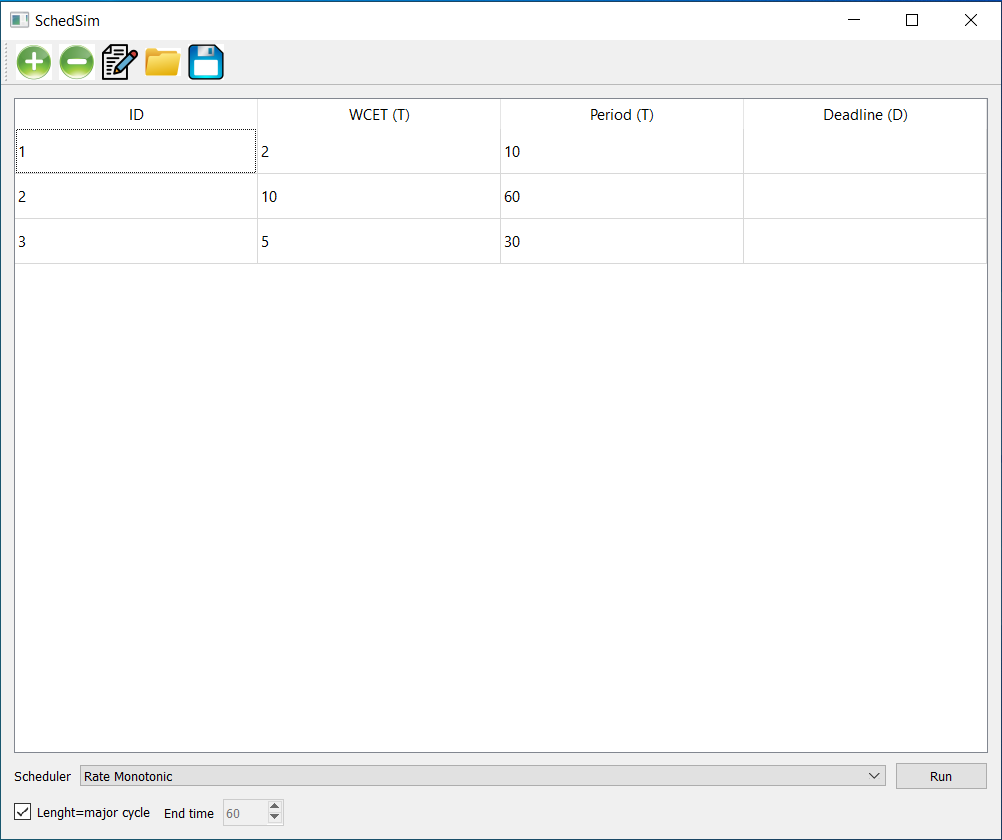
\includegraphics[width=1\textwidth]{main.png}
\caption{\label{fig:frog}Main page}
\end{figure}

\begin{figure}
\centering
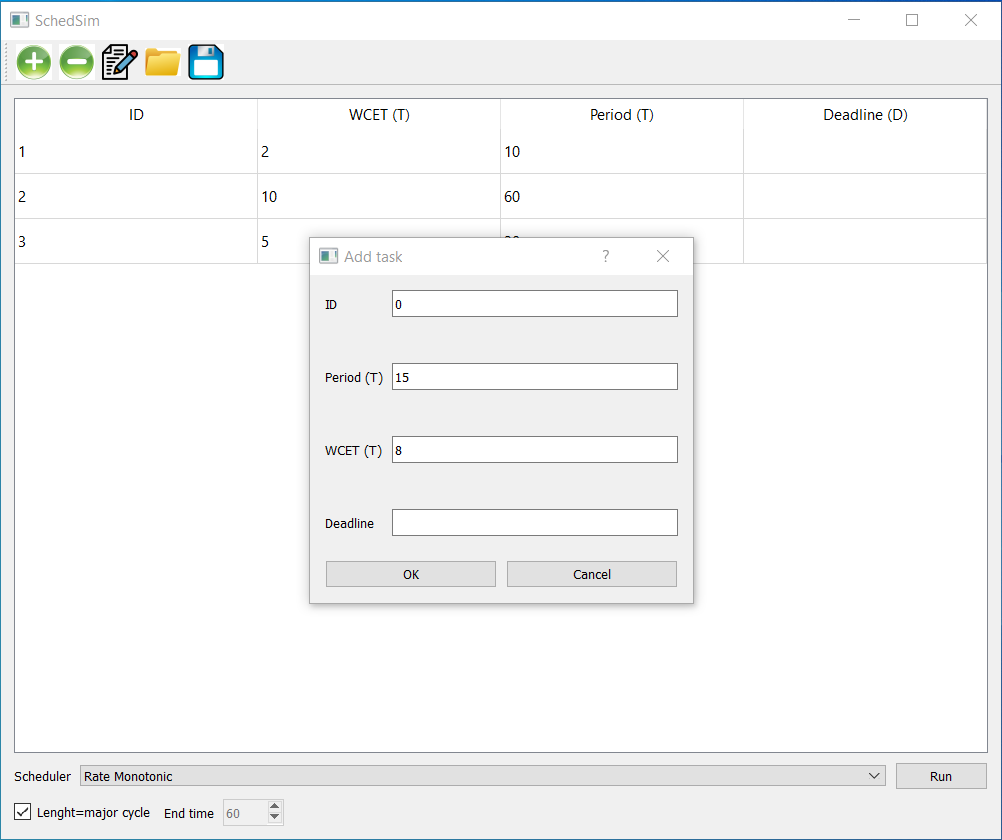
\includegraphics[width=1\textwidth]{add.png}
\caption{\label{fig:frog}Adding a task}
\end{figure}

\begin{figure}
\centering
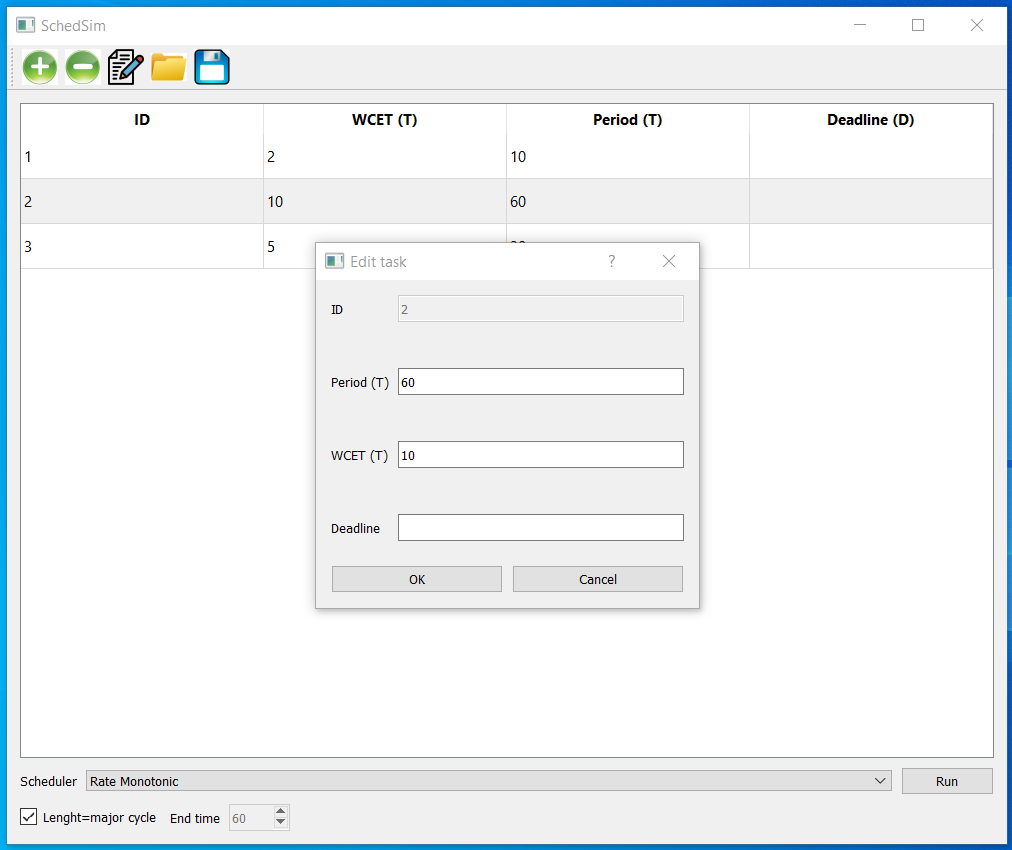
\includegraphics[width=1\textwidth]{edit.png}
\caption{\label{fig:frog}Editing a task}
\end{figure}

\begin{figure}
\centering
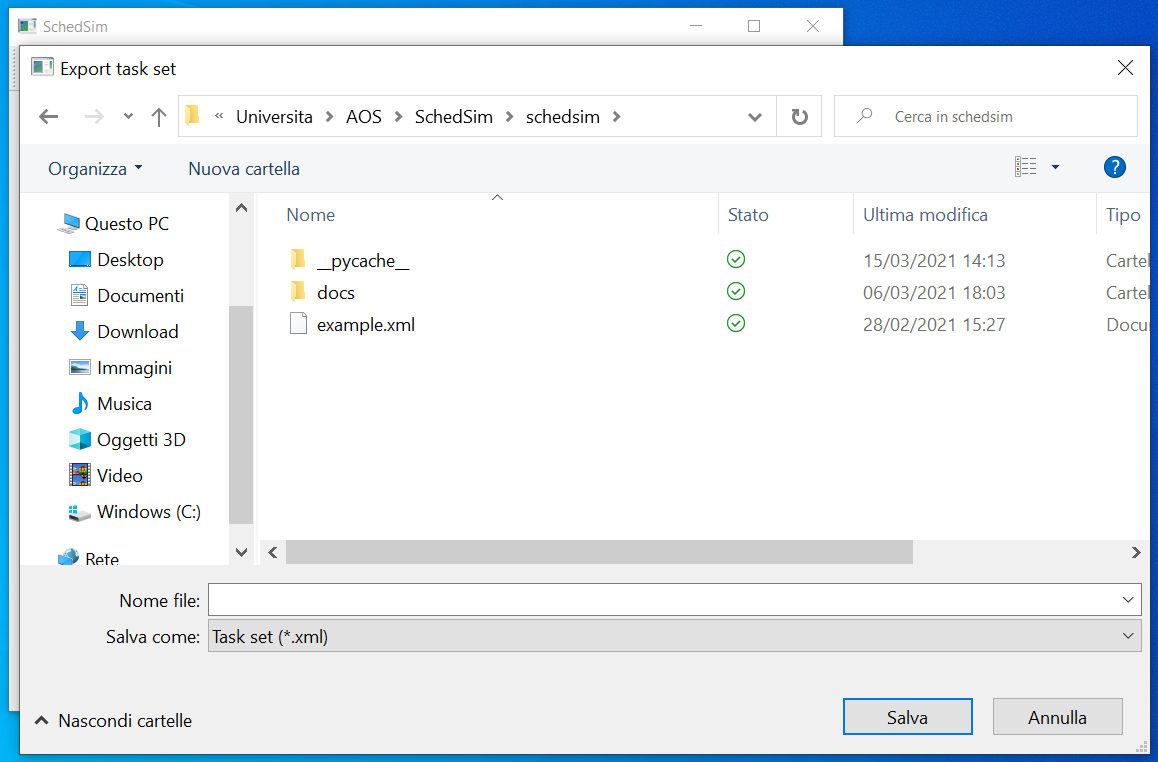
\includegraphics[width=1\textwidth]{export.png}
\caption{\label{fig:frog}Exporting a task set}
\end{figure}

\begin{figure}
\centering
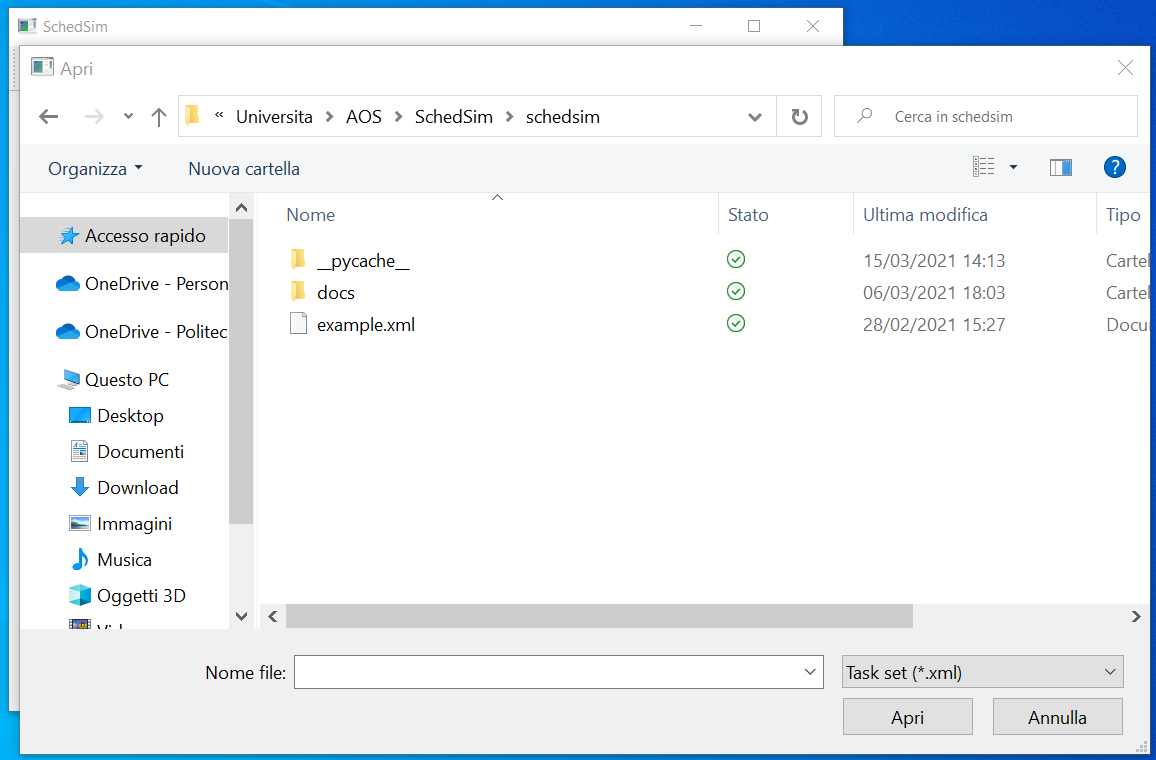
\includegraphics[width=1\textwidth]{import.png}
\caption{\label{fig:frog}Importing a task set}
\end{figure}

\begin{figure}
\centering
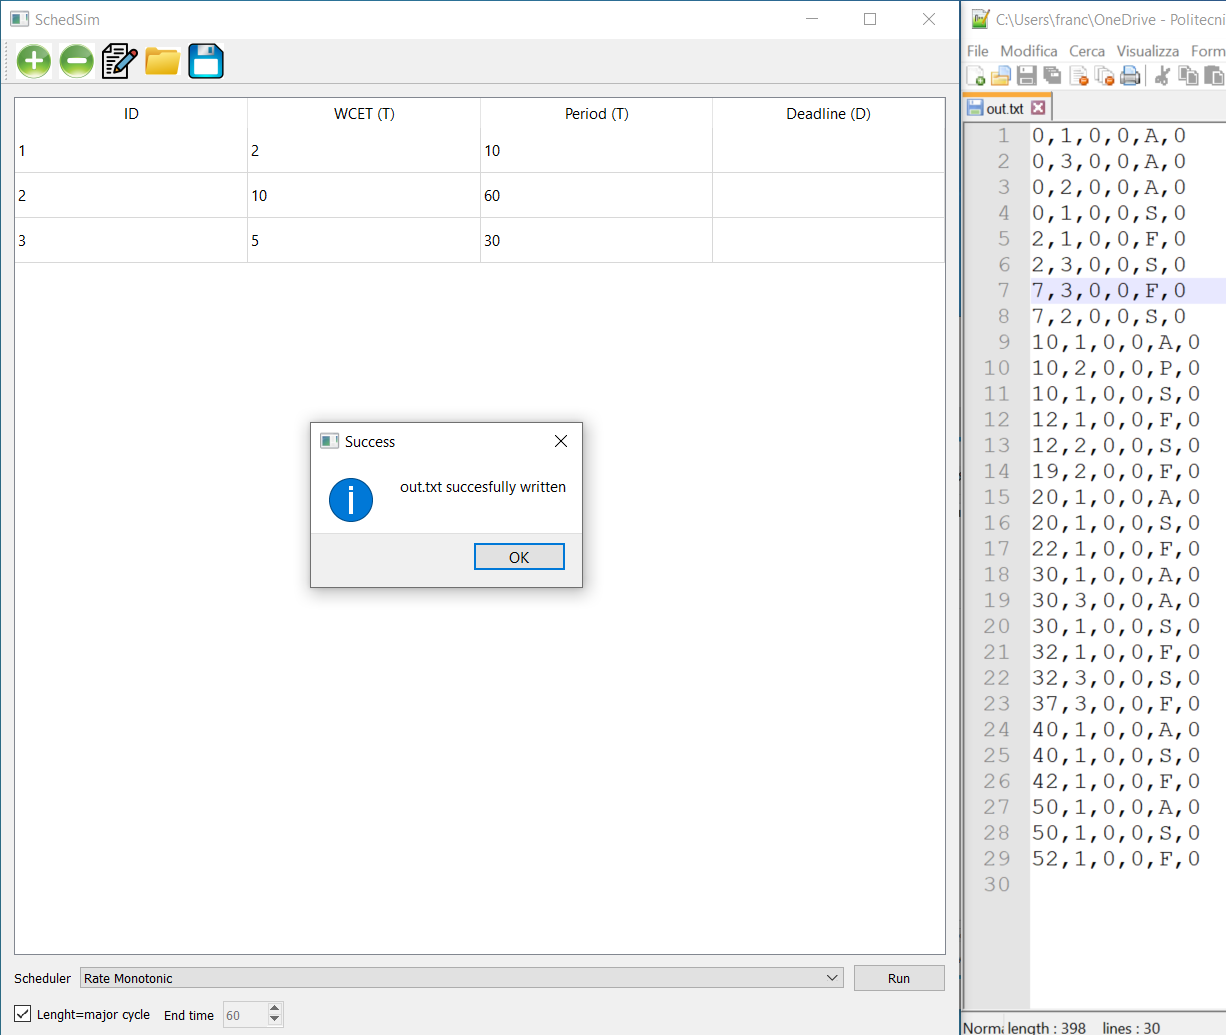
\includegraphics[width=1\textwidth]{success.png}
\caption{\label{fig:frog}Example of output given a task set, RateMonotonic scheduler}
\end{figure}

\end{document}